\chapter{Screenshots from deployment}

\begin{figure}[ht]
    \centering
    % This makes a box of 0pt width and puts the image in the center of it
    \makebox[\textwidth][c]{
        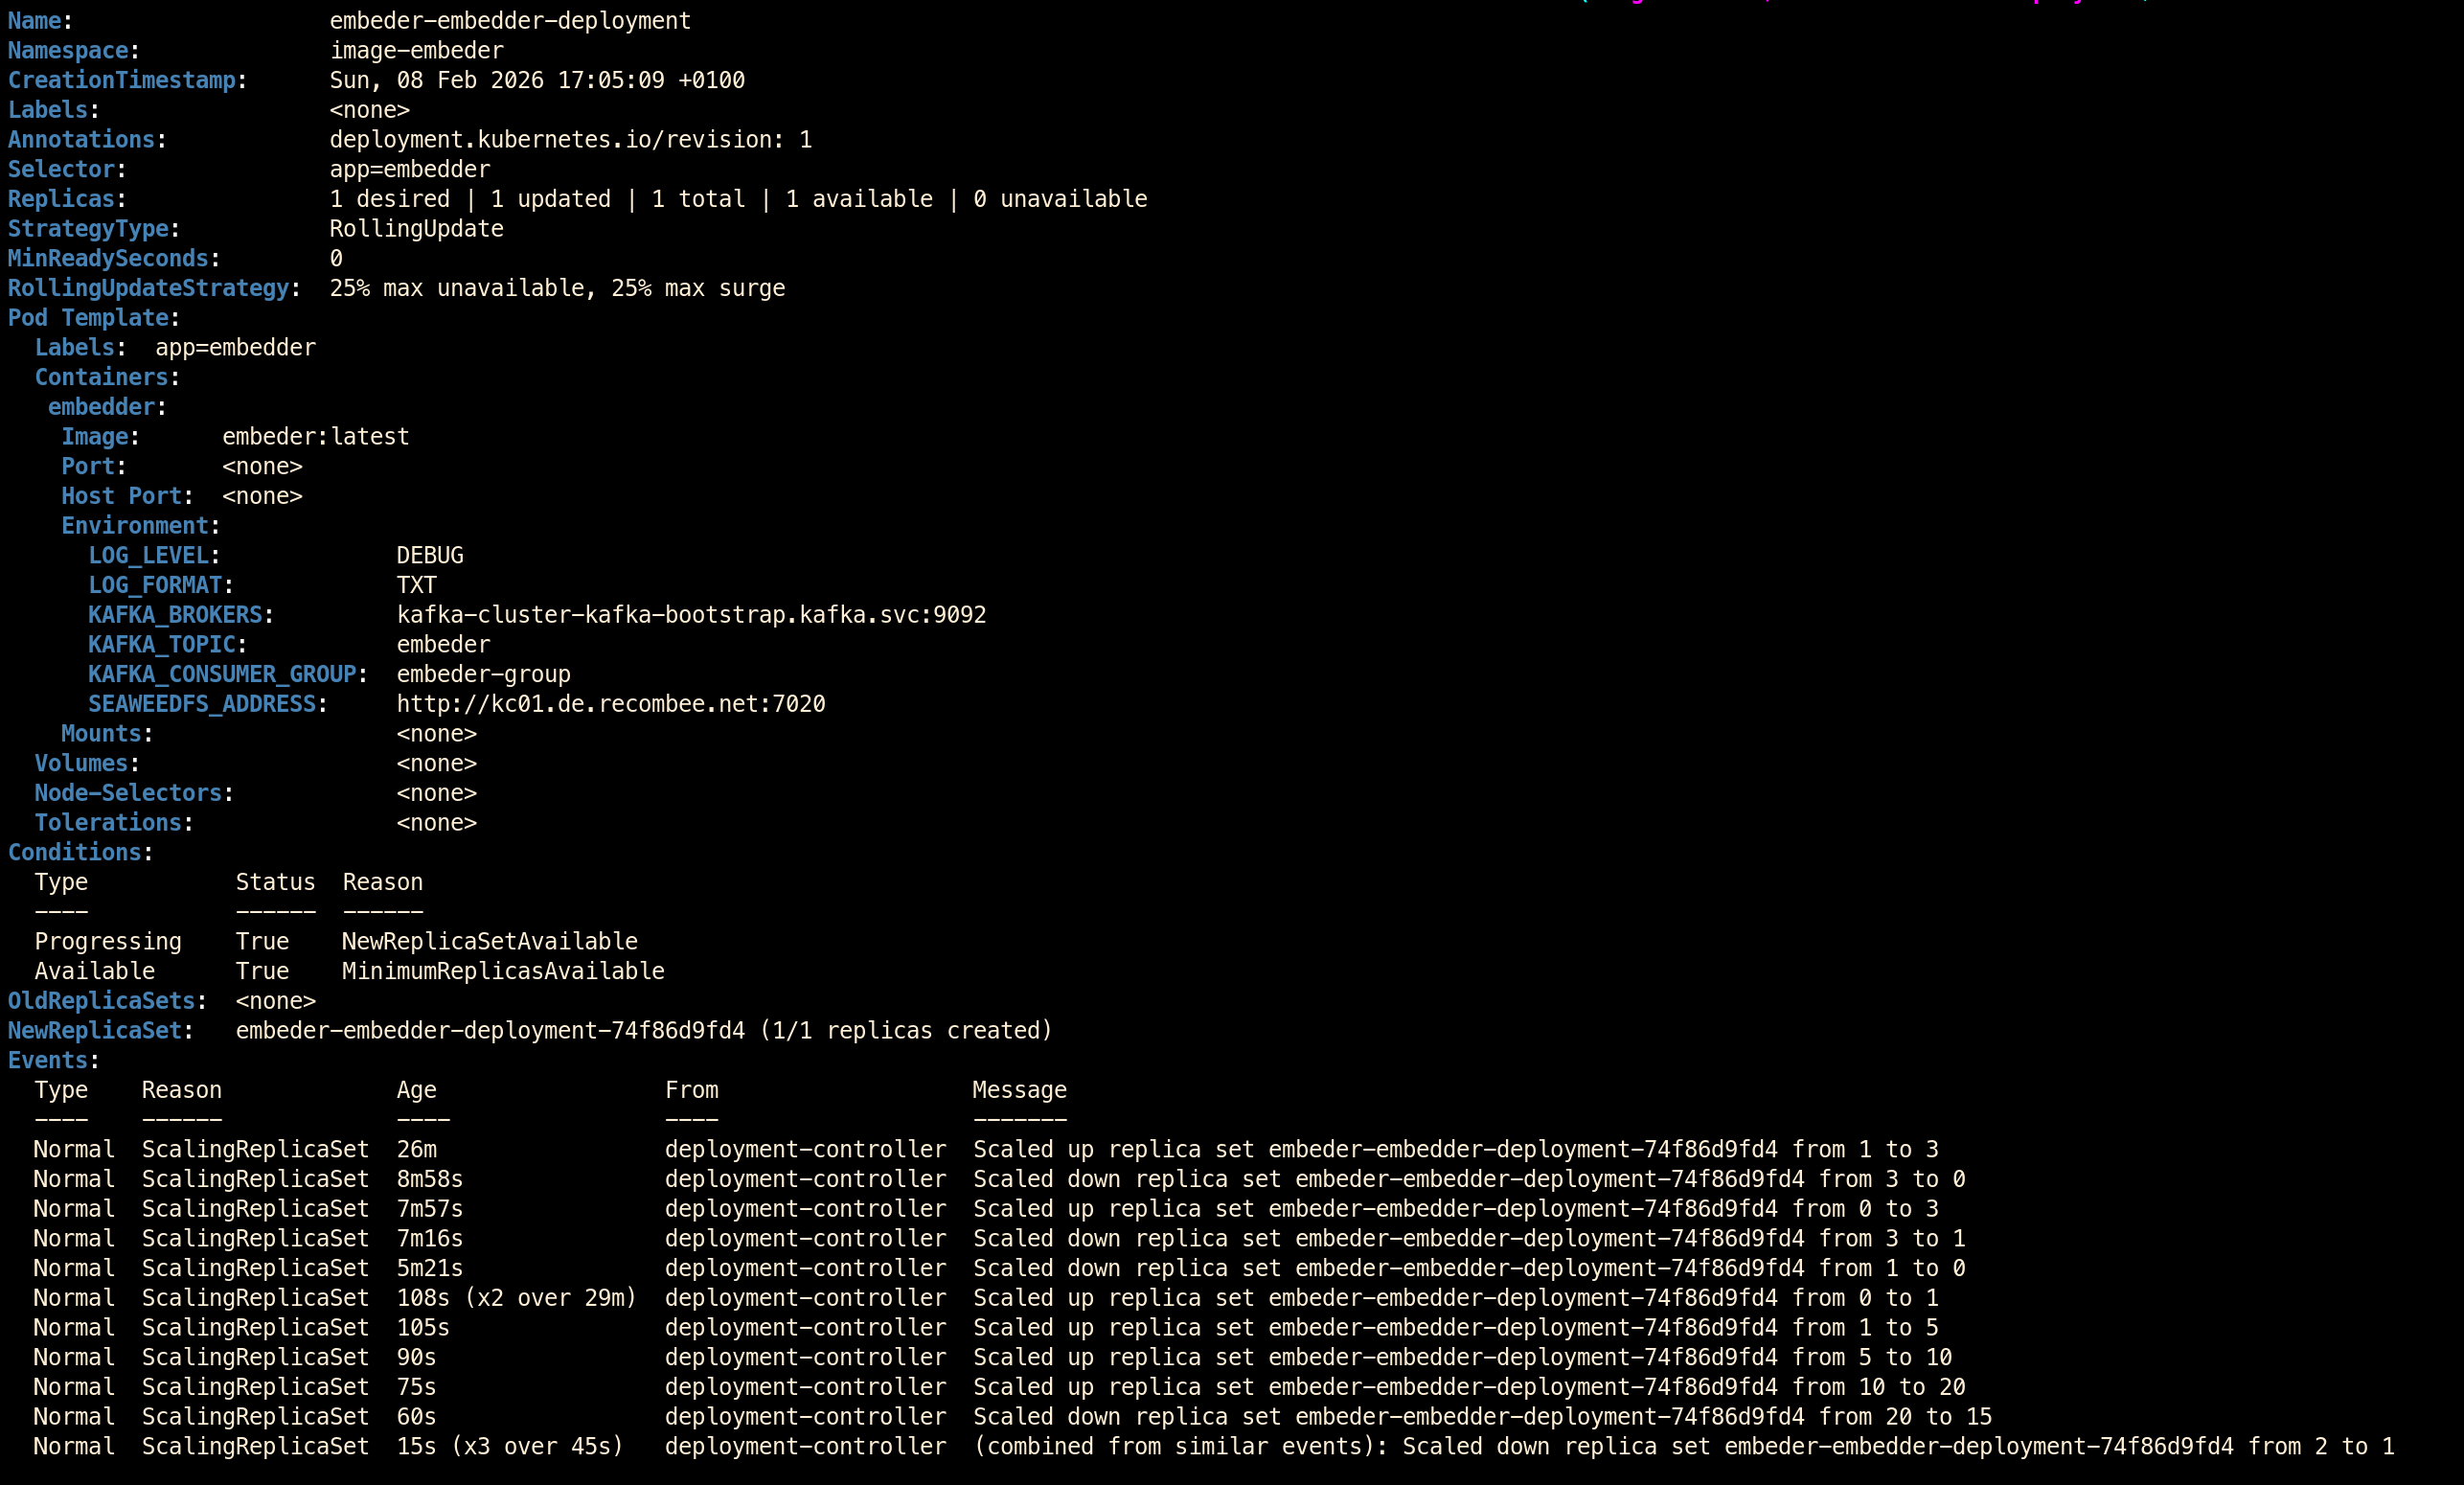
\includegraphics[width=0.85\paperwidth]{images/appendix/scalling.png}
    }
    \caption[Deployment scaling example]{Deployment scaling example. The screenshot contains events (bottom of the figure) of scaling the embedder component.}
\end{figure}


\begin{figure}[ht]
    \centering
    % This makes a box of 0pt width and puts the image in the center of it
    \makebox[\textwidth][c]{
        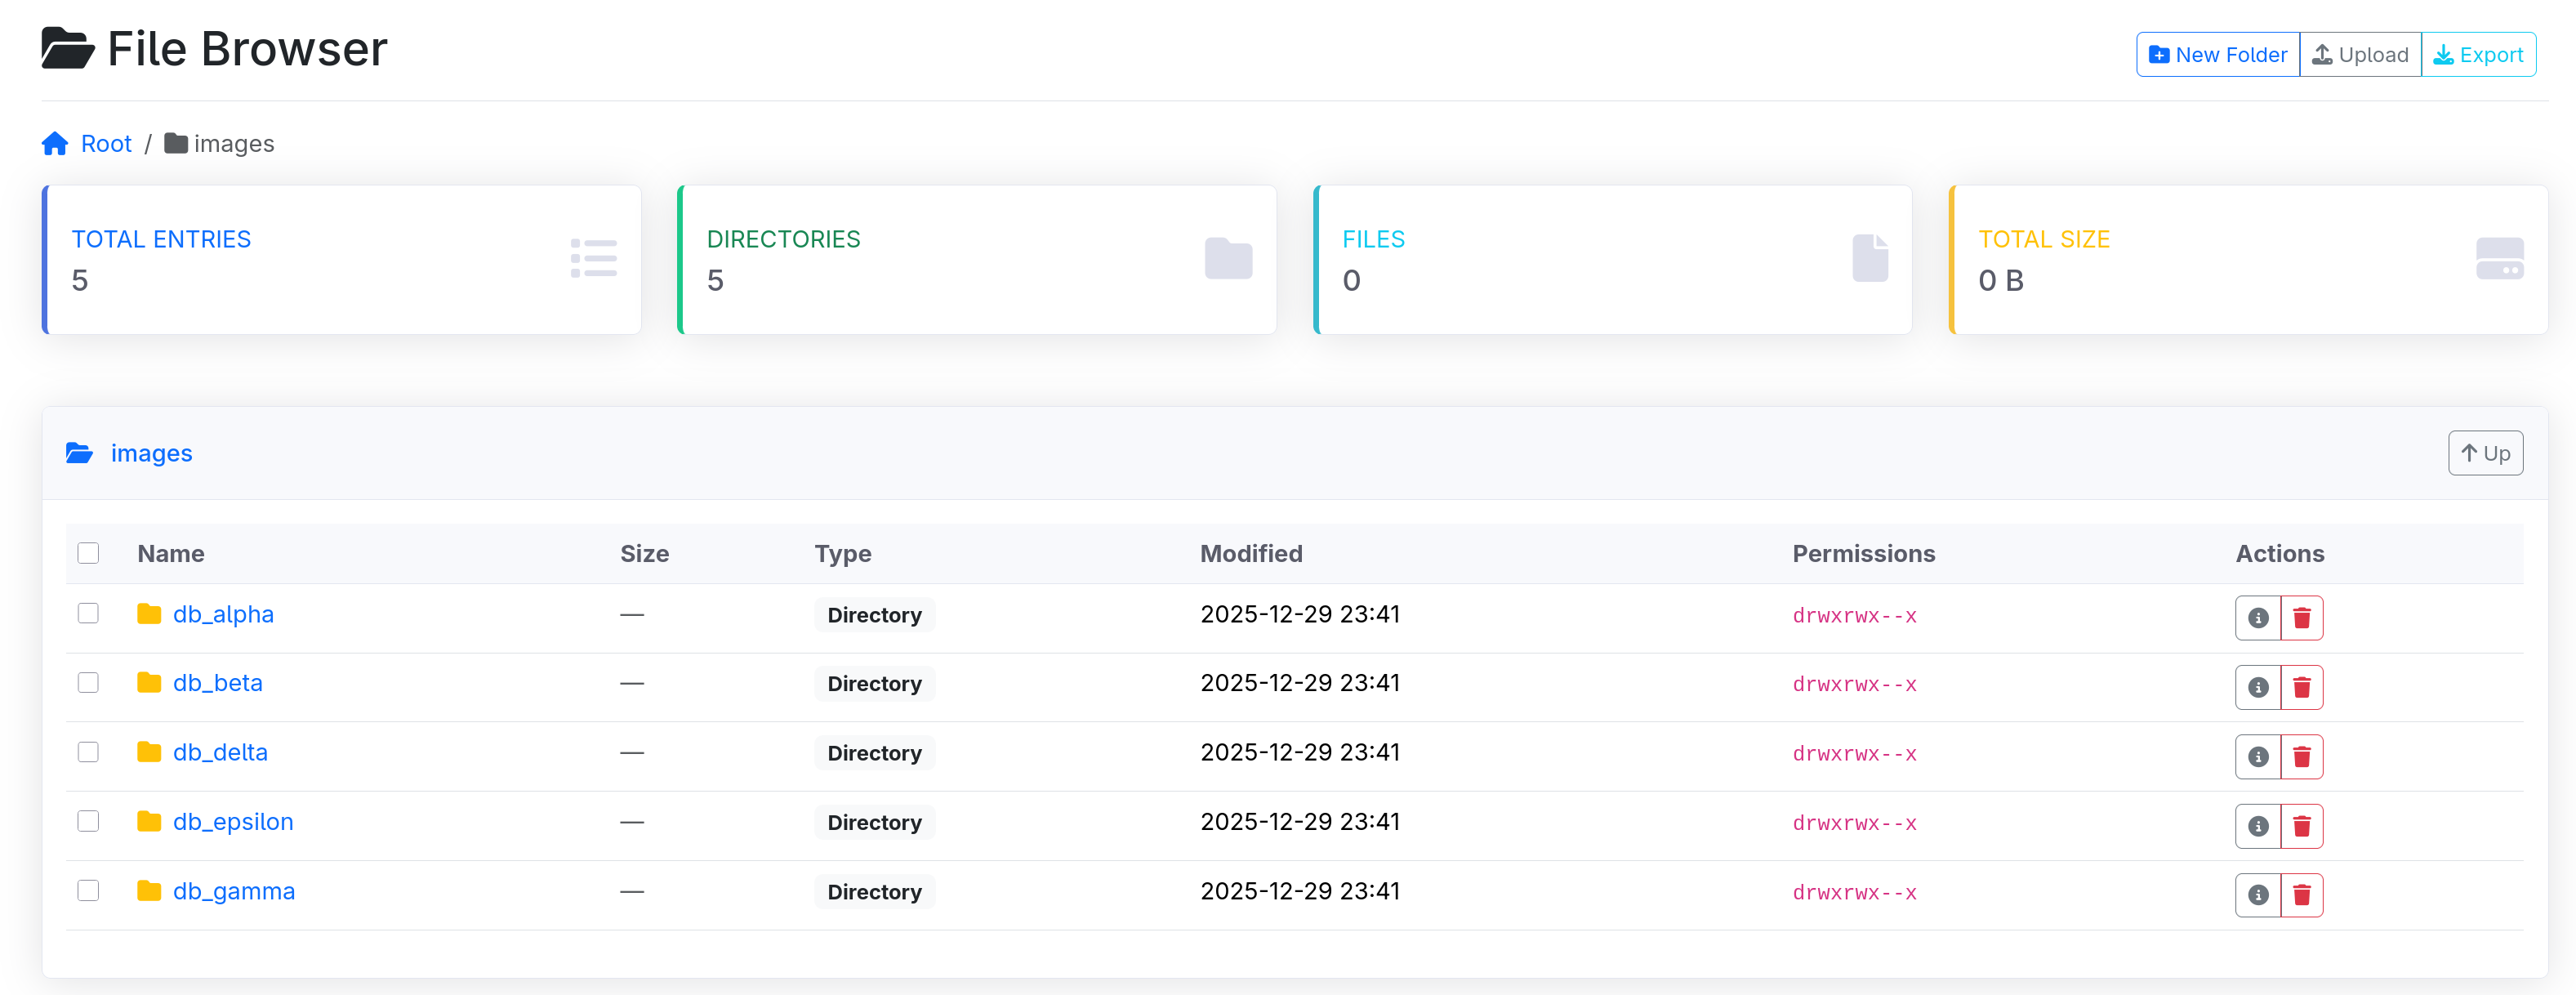
\includegraphics[width=0.85\paperwidth]{images/appendix/image.png}
    }
    \caption[Filler UI]{Filler UI. Web UI for interacting with filer. The web interface can be used to list, upload, delete files, and manage basic storage metadata.}
\end{figure}



\begin{figure}[ht]
    \centering
    % This makes a box of 0pt width and puts the image in the center of it
    \makebox[\textwidth][c]{
        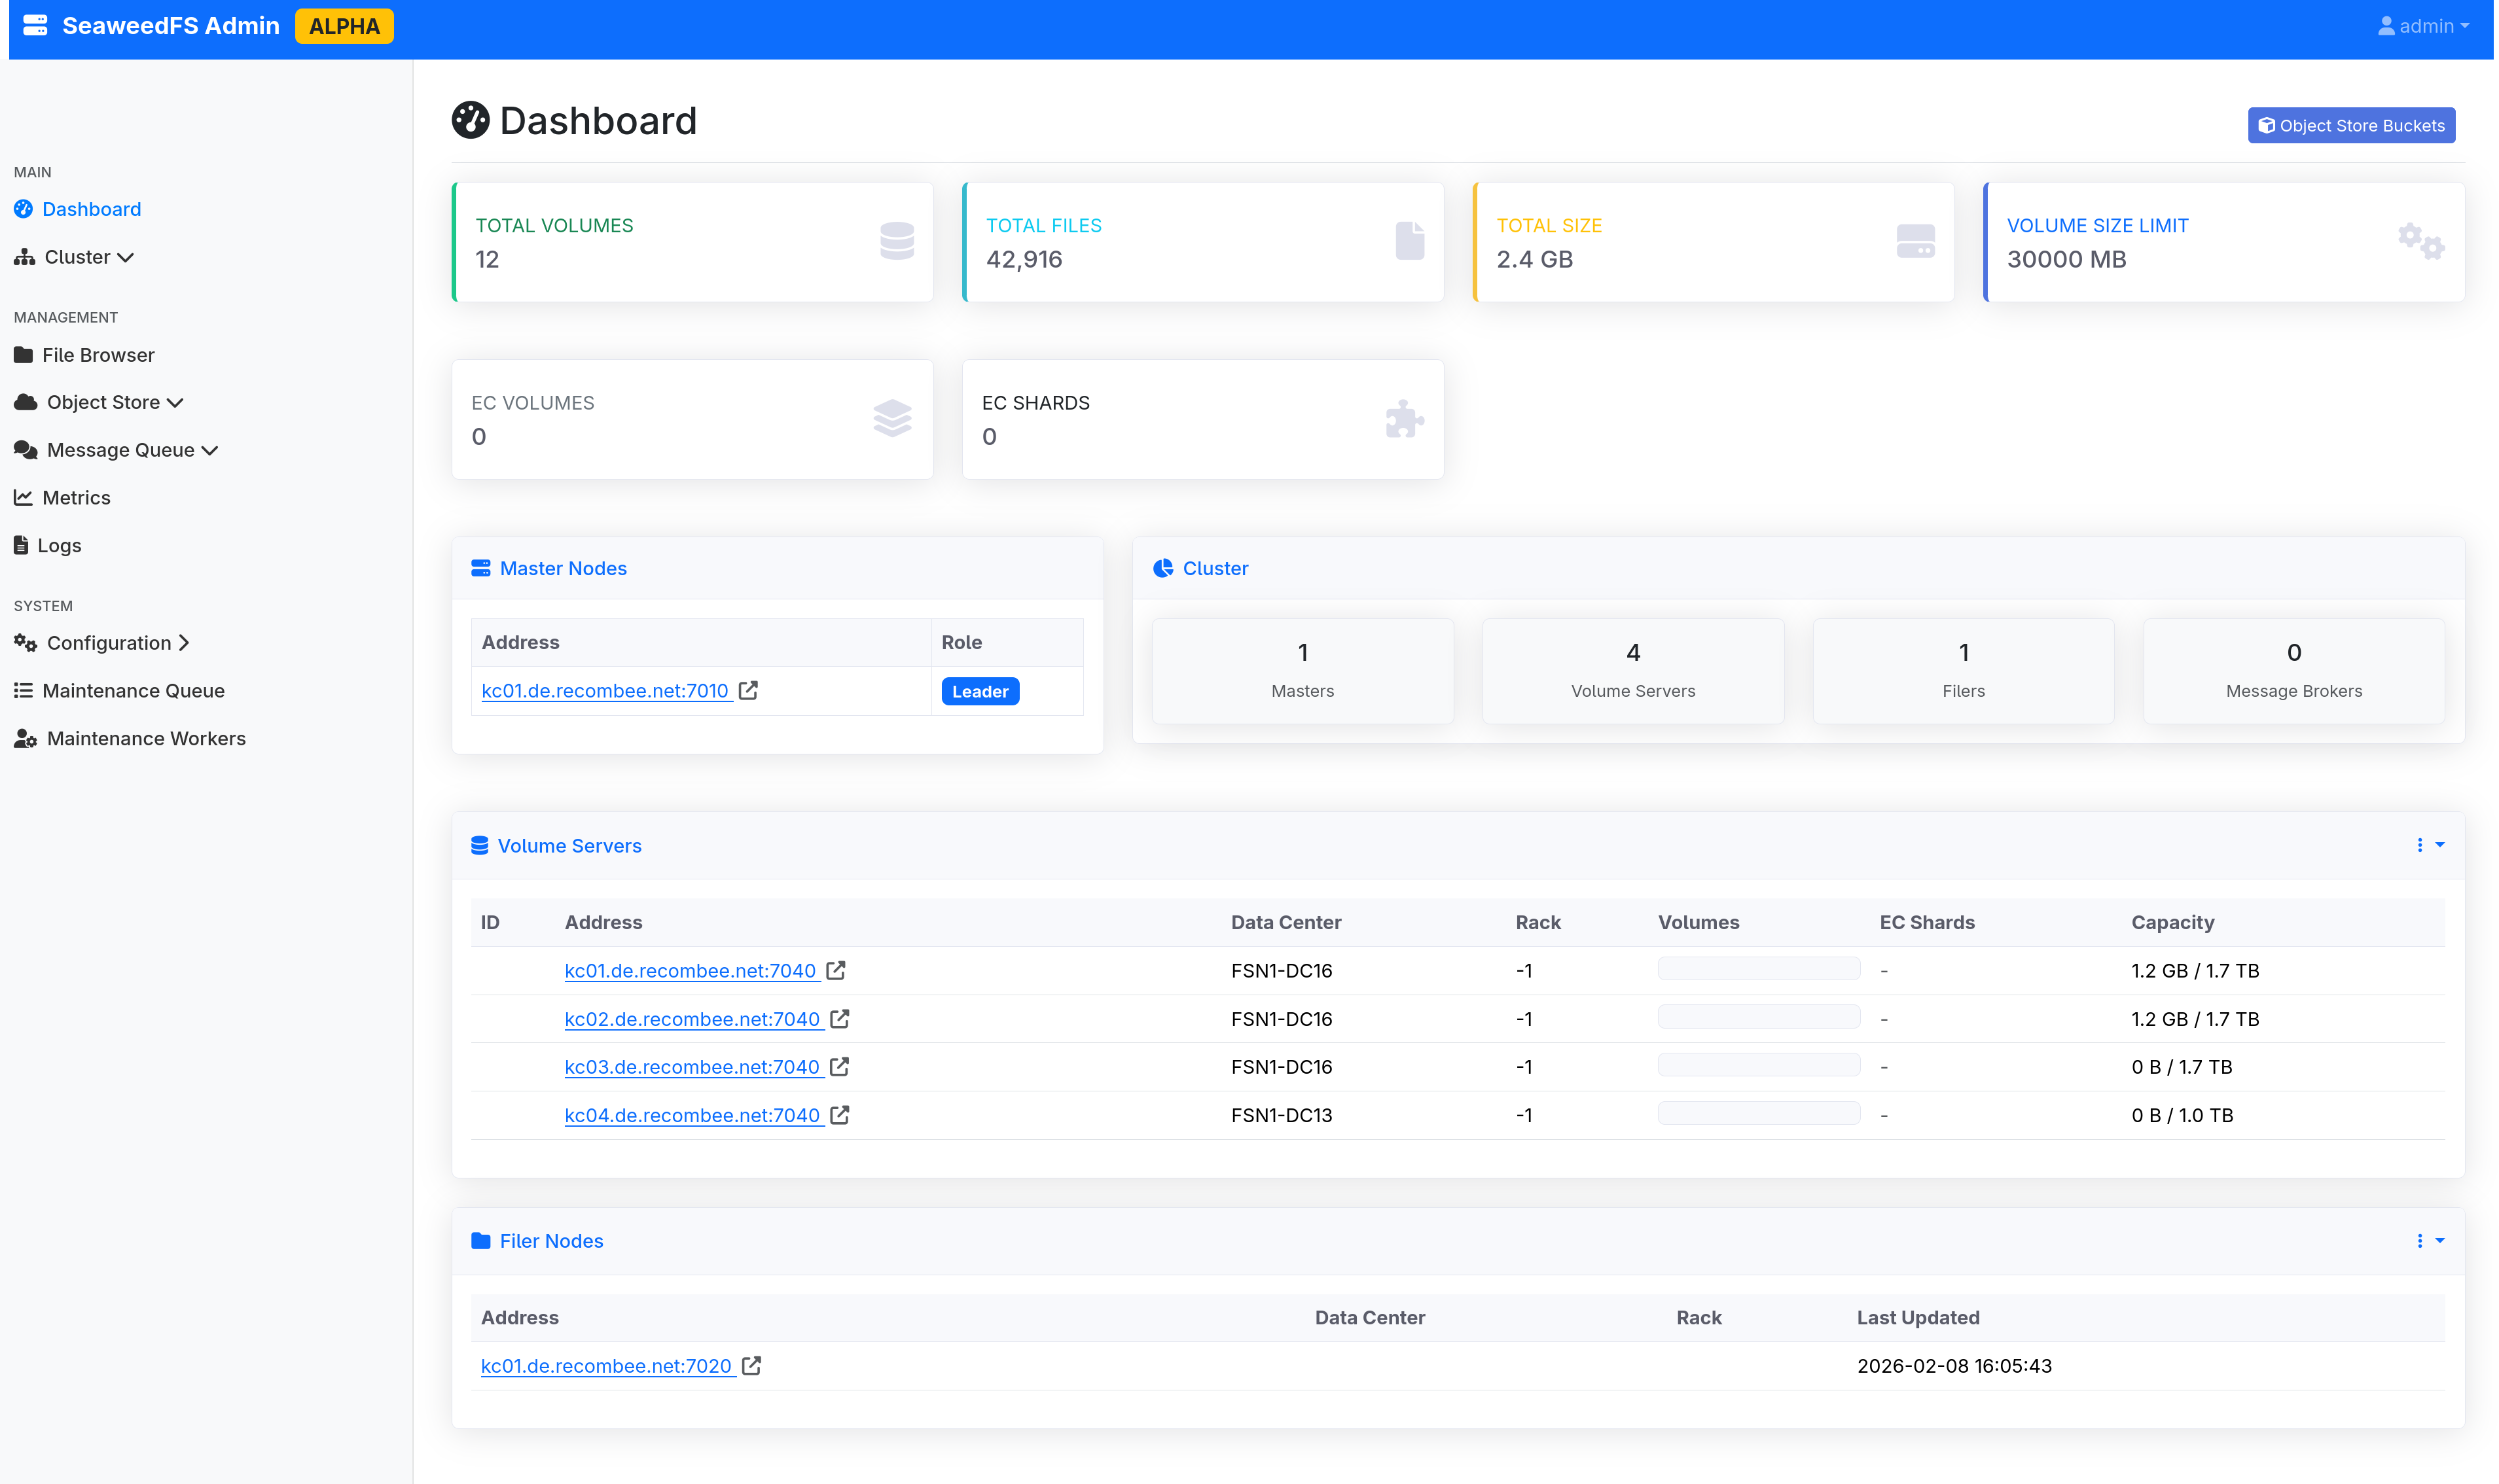
\includegraphics[width=0.85\paperwidth]{images/appendix/seaweed-API.png}
    }
    \caption{SeaweedFS admin UI}
\end{figure}


\begin{figure}[ht]
    \centering
    % This makes a box of 0pt width and puts the image in the center of it
    \makebox[\textwidth][c]{
        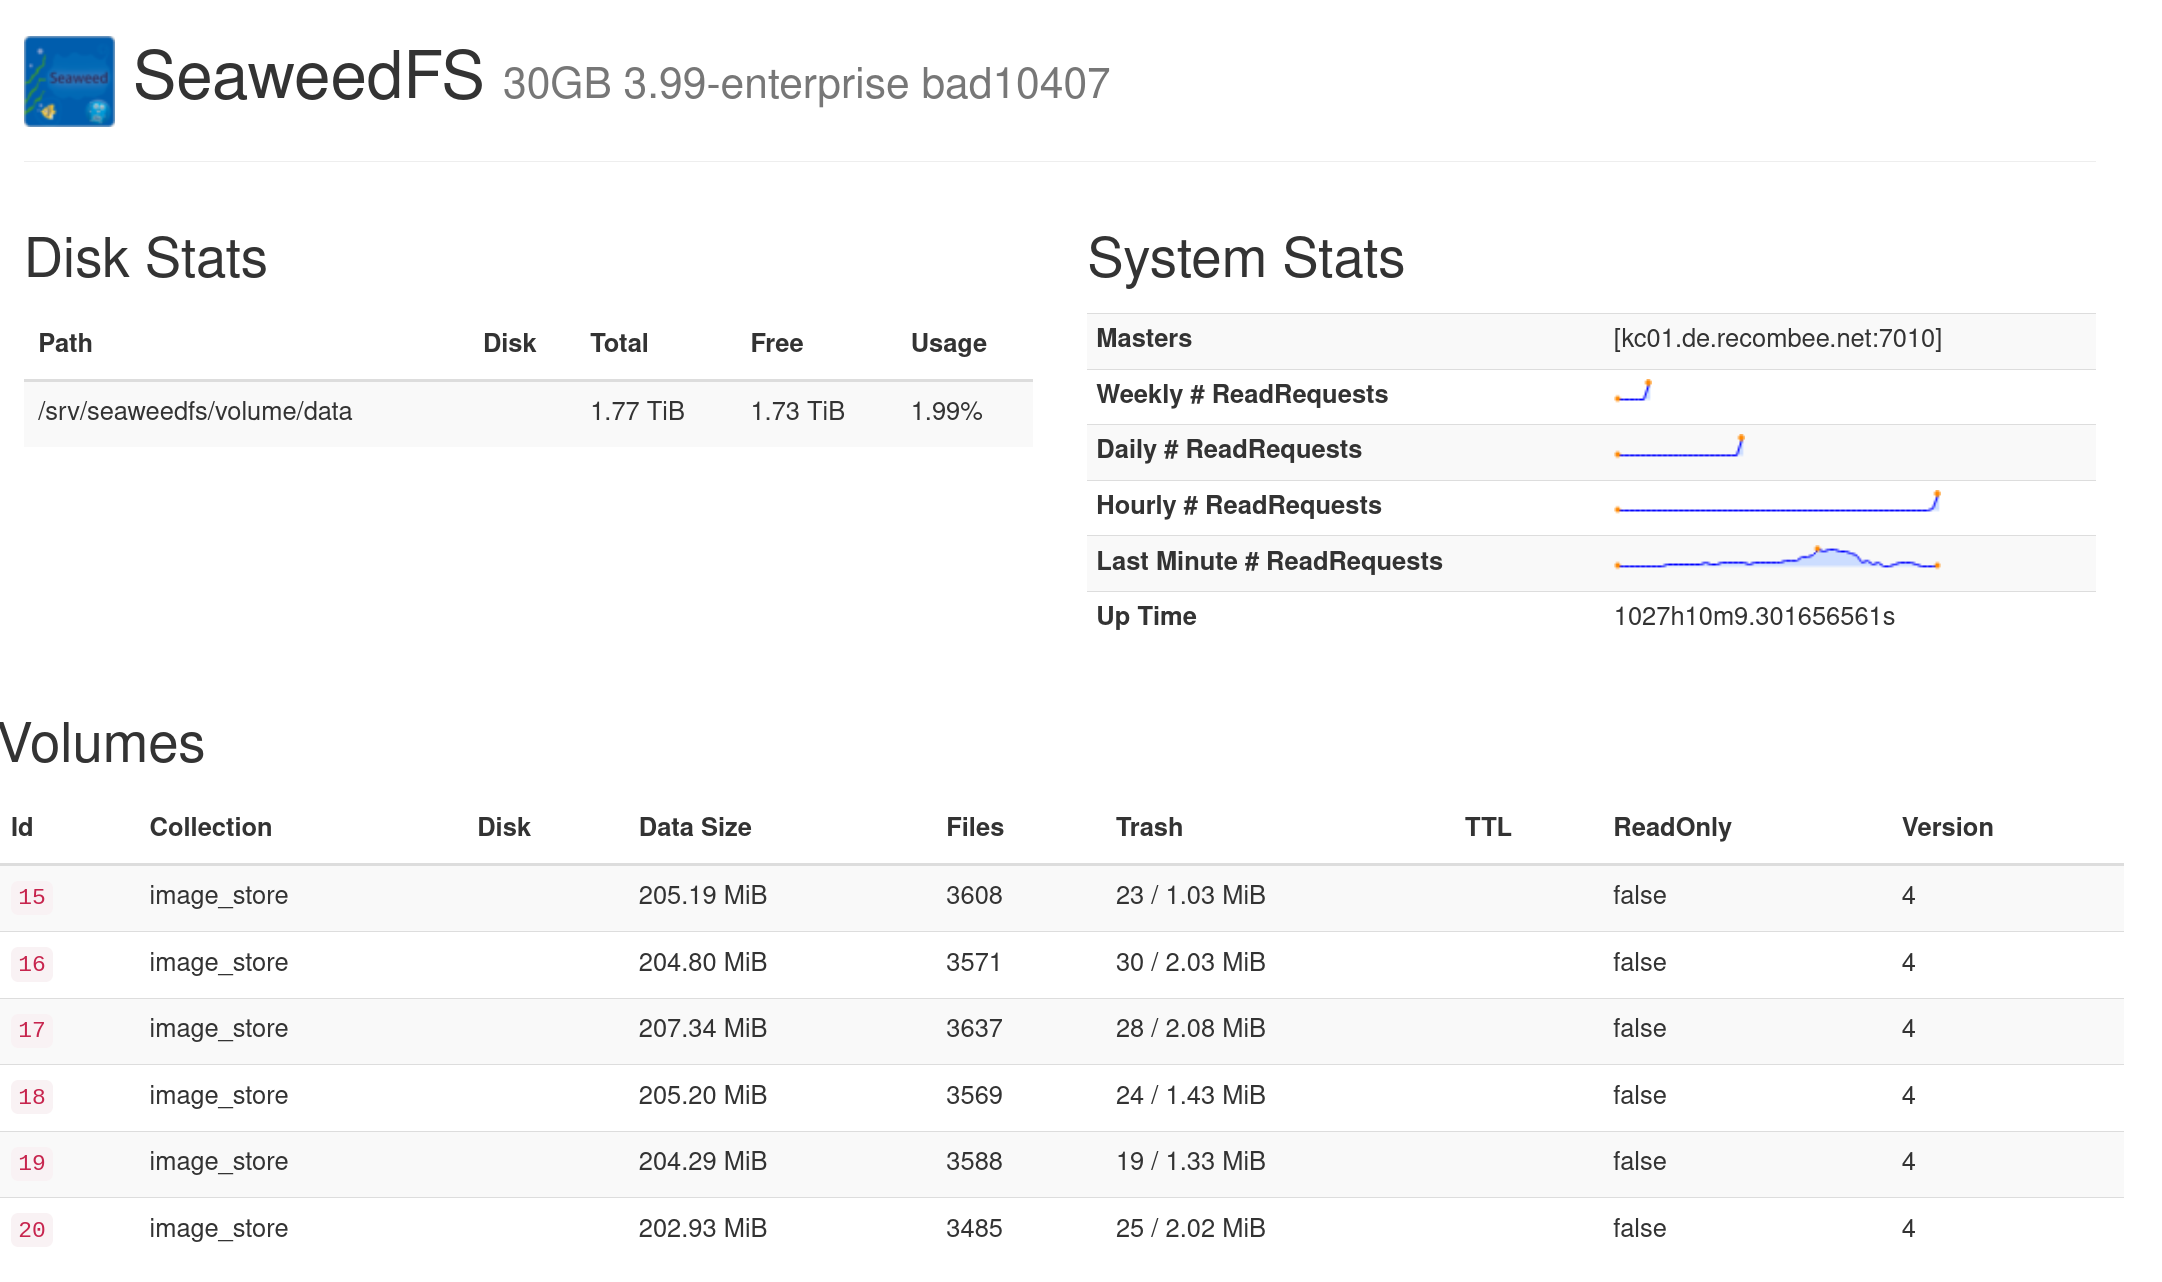
\includegraphics[width=0.85\paperwidth]{images/appendix/wolumeserverUI.png}
    }
    \caption{Volume server web UI}
\end{figure}

\begin{figure}[ht]
    \centering
    % This makes a box of 0pt width and puts the image in the center of it
    \makebox[\textwidth][c]{
        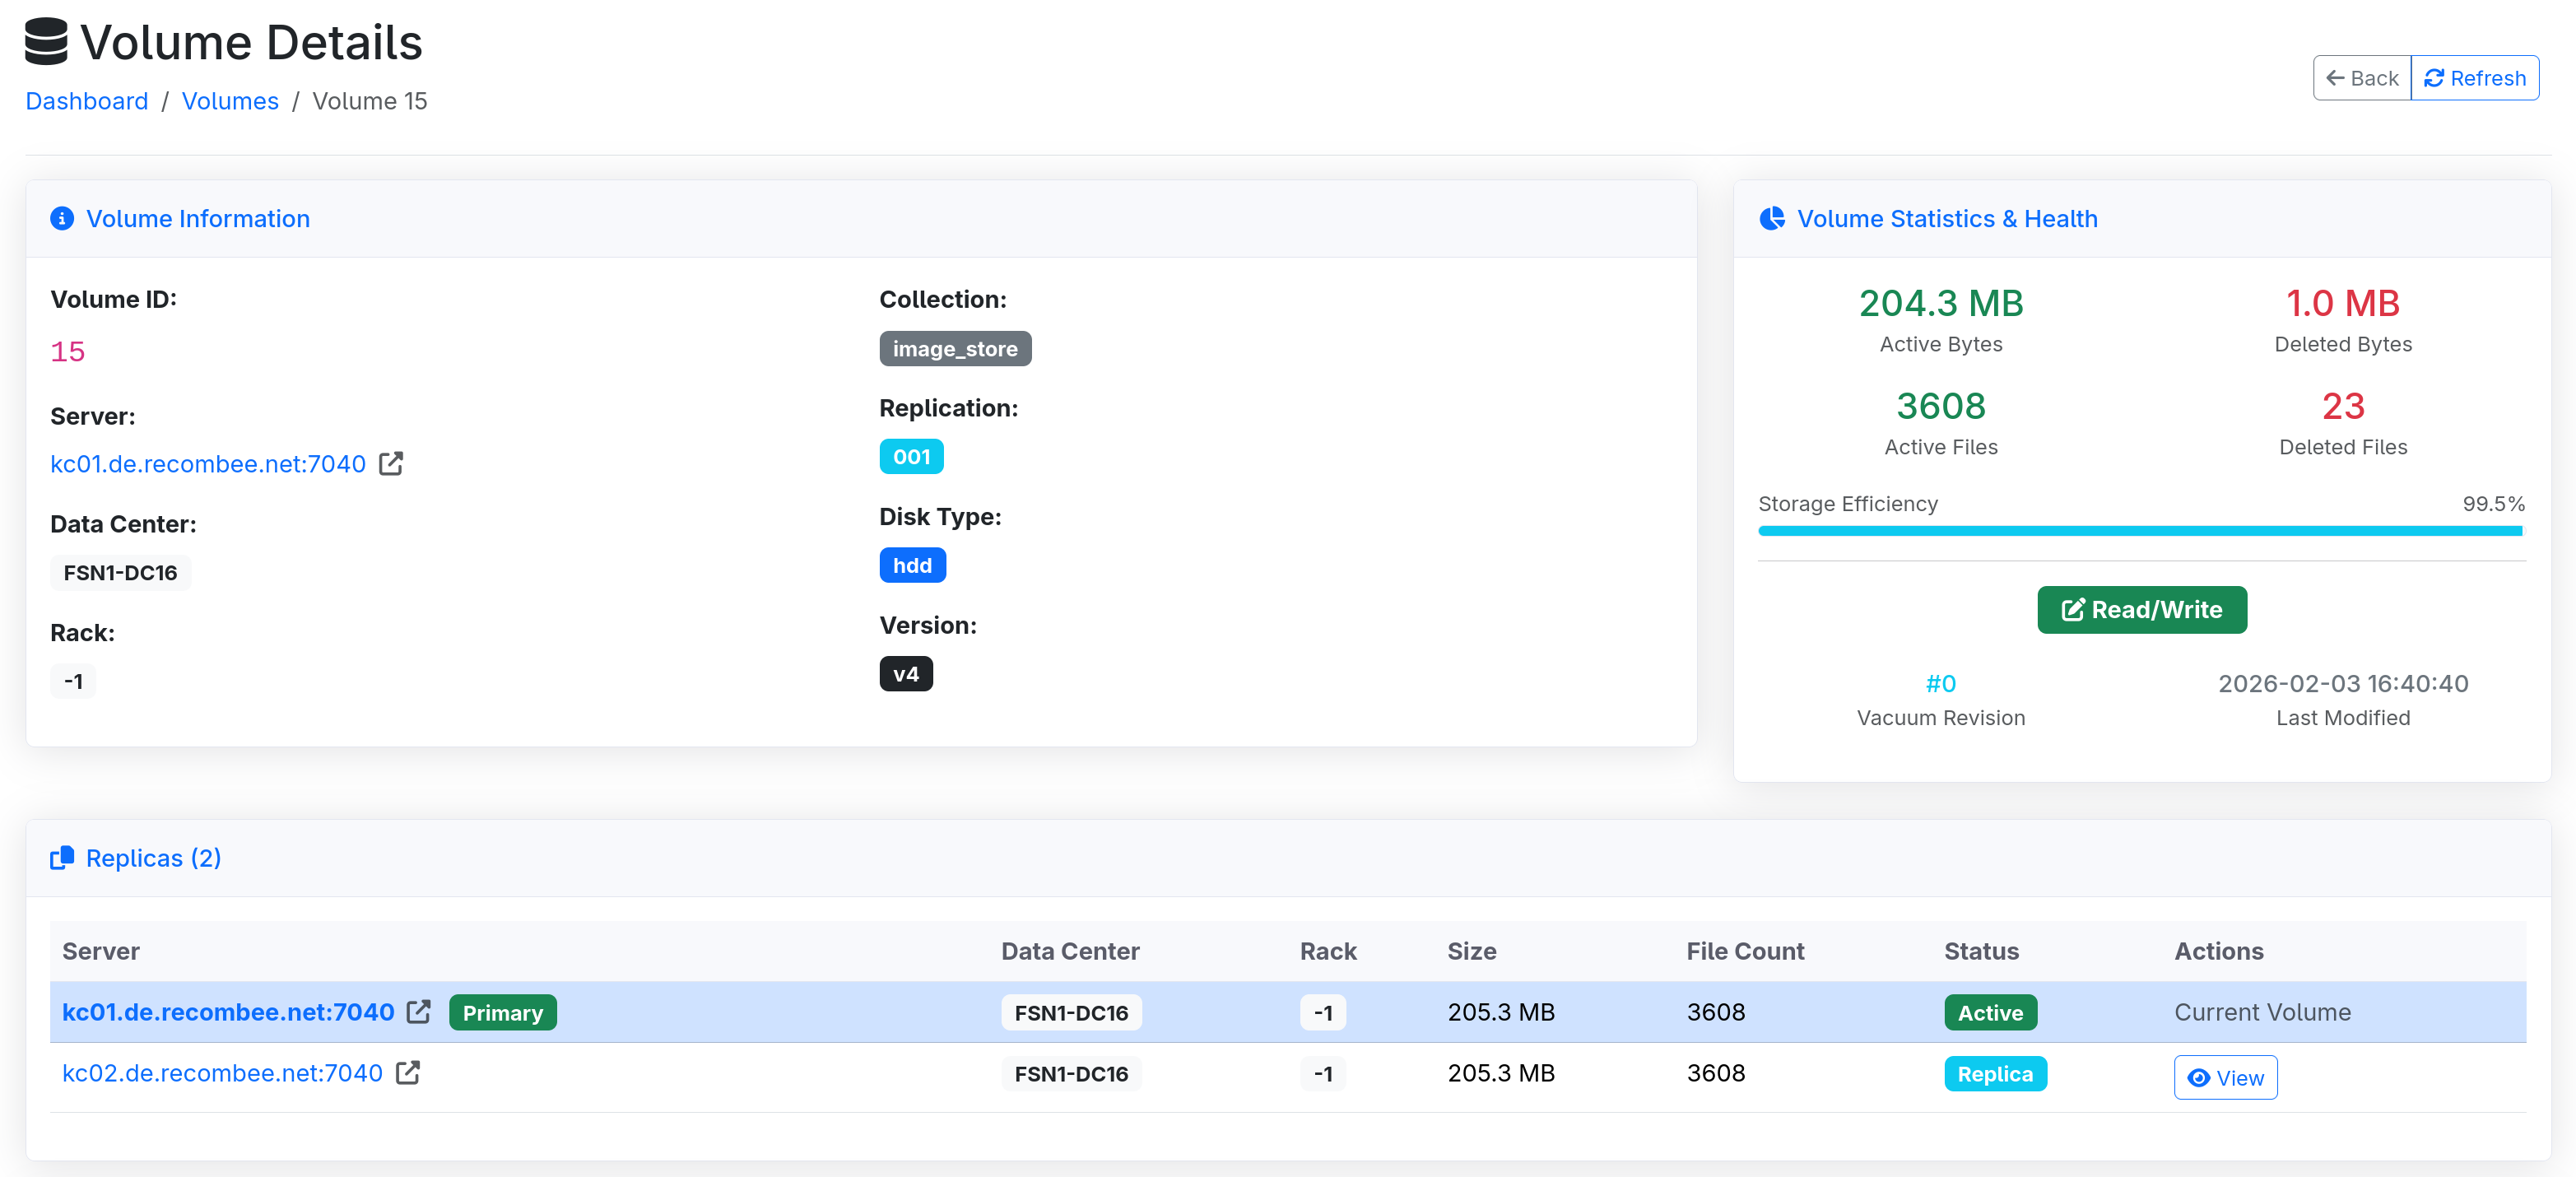
\includegraphics[width=0.85\paperwidth]{images/appendix/wolumeUI.png}
    }
    \caption{Volume UI}
\end{figure}

\begin{figure}[ht]
    \centering
    % This makes a box of 0pt width and puts the image in the center of it
    \makebox[\textwidth][c]{
        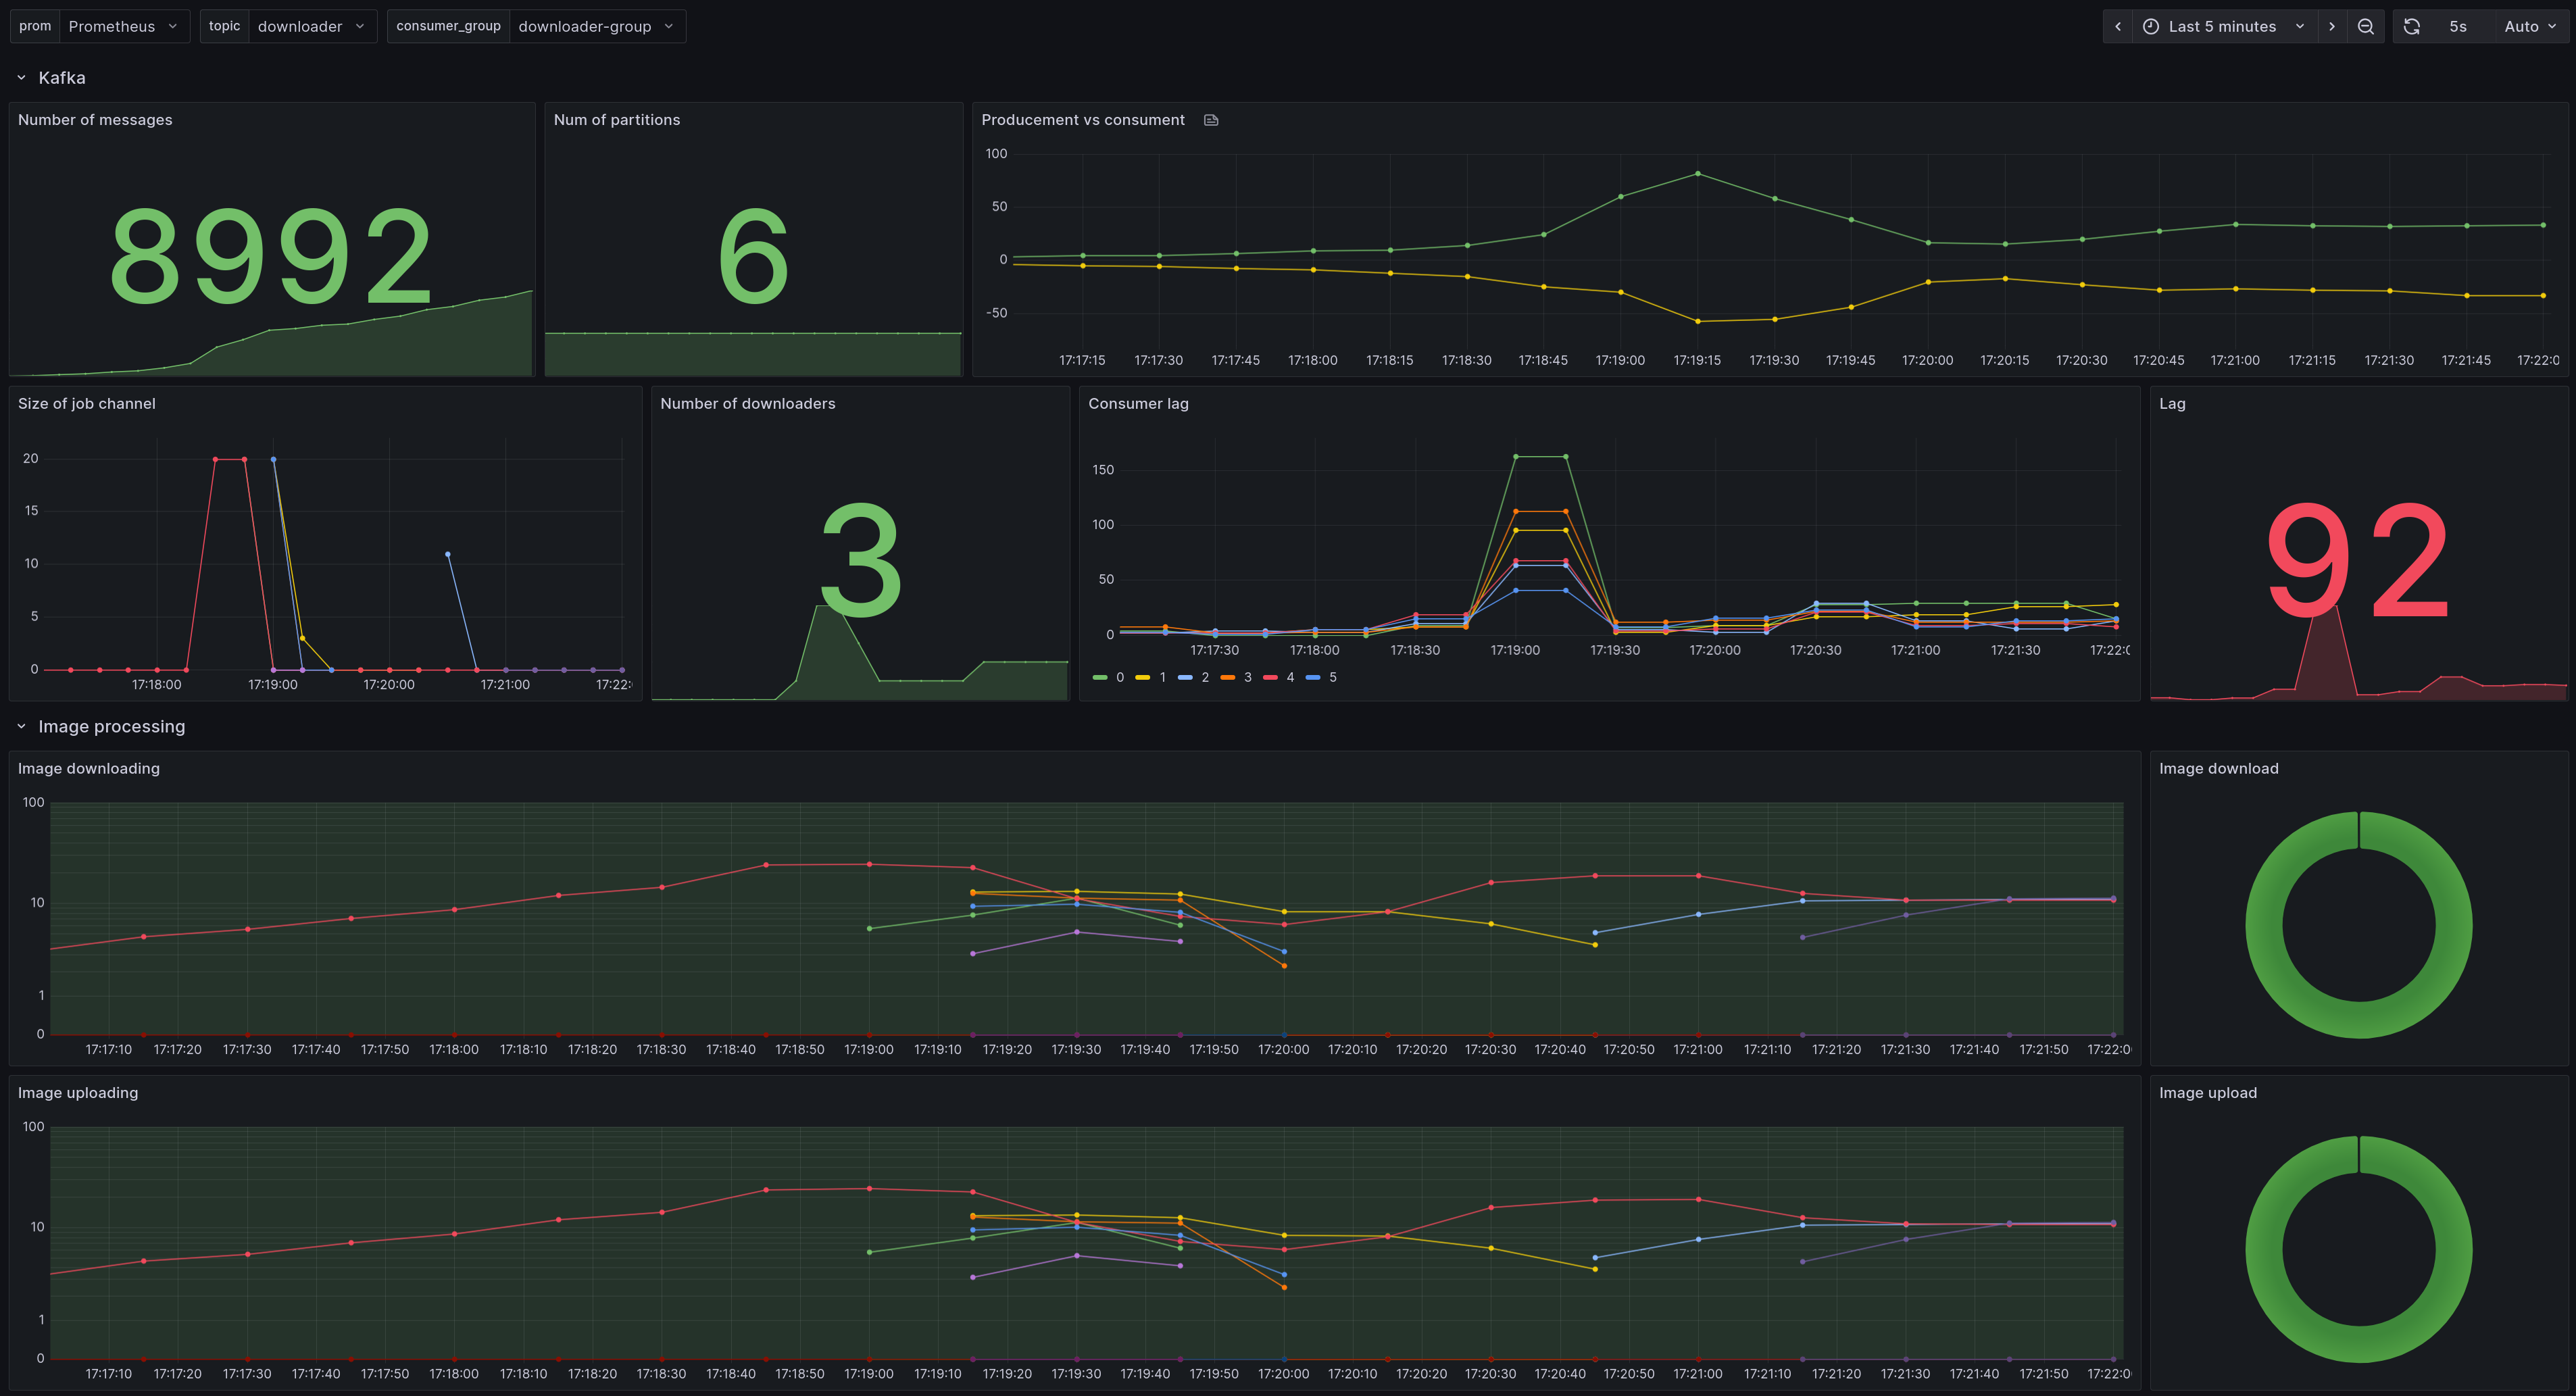
\includegraphics[width=0.85\paperwidth]{images/appendix/grafana.png}
    }
    \caption[Grafana Dowloader dashboard]{Downloader Grafana dashboard. The dashboard displays metrics from Kafka, Image Reactor, and Downloader. From top left: \textit{Number of messages}, \textit{Number of partitions}, \textit{Producer vs consumer}, \textit{Size of job channel}, \textit{Number of downloaders}, \textit{Consumers lag}, \textit{Lag}, \textit{Image downloading}, \textit{Image downloaded}, \textit{Image uploading}, \textit{Image uploaded}.}
\end{figure}

\begin{figure}[ht]
    \centering
    % This makes a box of 0pt width and puts the image in the center of it
    \makebox[\textwidth][c]{
        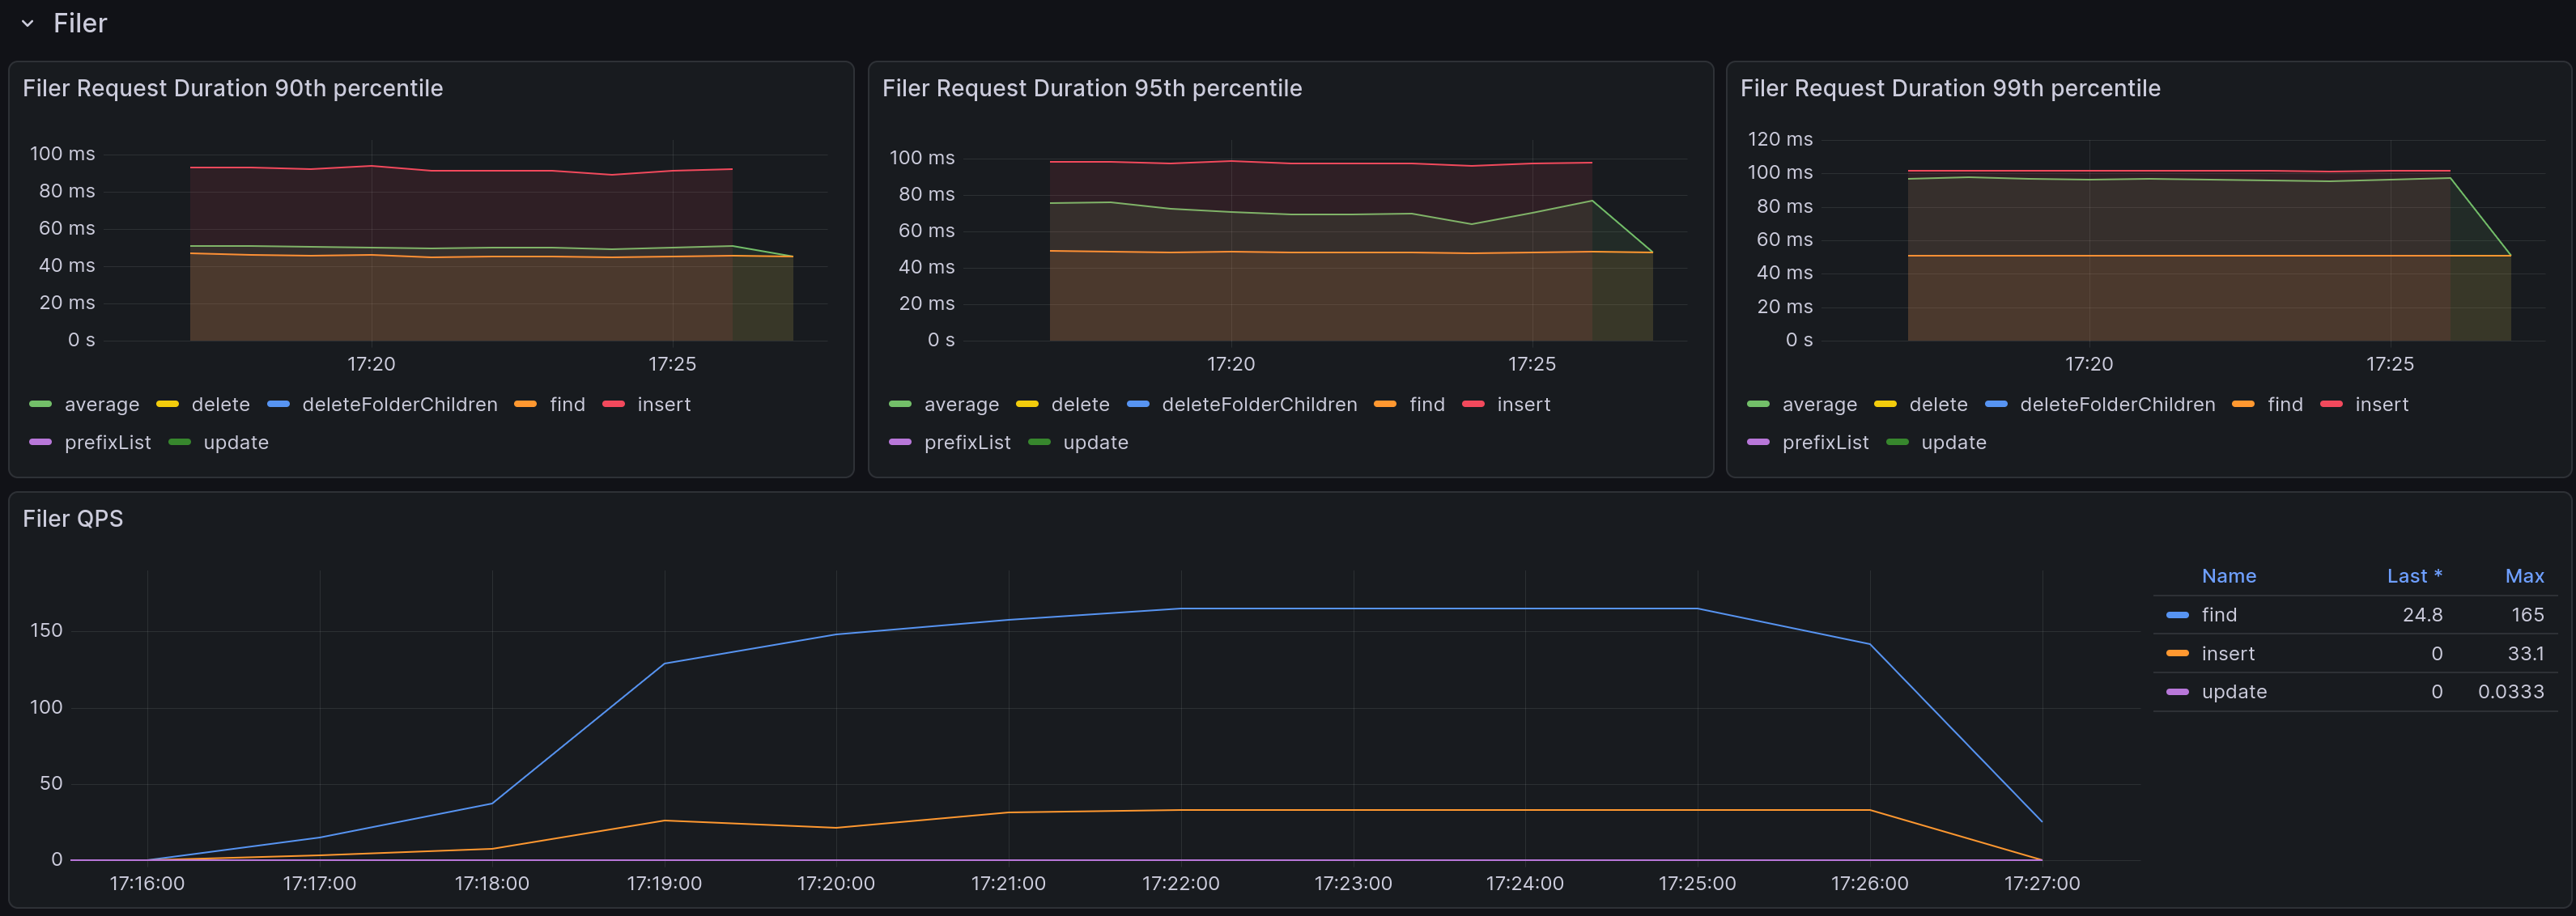
\includegraphics[width=0.85\paperwidth]{images/appendix/seaweedfs_grafana.png}
    }
    \caption[Grafana SeaweedFS dashboard]{SeaweedFS Grafana dashboard. From top left: \textit{Filer Request Duration 90th percentile}, \textit{Filer Request Duration 95th percentile}, \textit{Filer Request Duration 99th percentile}, \textit{Filer QPS}}
\end{figure}